\documentclass[a4paper, 10pt]{article} %titlepage reseta a numeração da capa e quebra a página.


%pacotes que serão usados======================================================================================
\usepackage[portuges, brazil]{babel}
\usepackage[utf8x]{inputenc} %Acentuação automática
%\usepackage[T1]{fontenc} %Muda a codificação do texto, tornando possível cópia com acentos.
\usepackage[active]{srcltx}
\usepackage{amsfonts,amscd,bezier,amssymb} %Pacotes matemáticos
\usepackage{amsmath, amsthm} %Outros pacotes matemáticos
\usepackage[mathscr]{eucal} %Outros pacotes matemáticos
\usepackage[dvips]{graphicx} %Pacotes para carragamento de imagens
\usepackage{indentfirst} %Identa automaticamente todo primeiro parágrafo
\usepackage{algpseudocode} %Pacote de algoritmos
\usepackage[ruled]{algorithm} %Pacote de algoritmos
\usepackage{algorithmicx} %Pacote de algoritmo
\usepackage{listings} %Implementações C
\usepackage{color}
\usepackage[justification=centering]{caption}
\usepackage{enumitem}
\usepackage{subfig}
\usepackage{cite} %Pacote para citação de bibliografia
\usepackage{url} %URL de sites na bibliografia
\usepackage{numprint}
\usepackage{multicol}
%\usepackage[pdftex, colorlinks=false, pdfborder={0 0 0}, plainpages=false, bookmarks=true, unicode = true]{hyperref}
%==============================================================================================================

%Definição de cores============================================================================================
\definecolor{dkgreen}{rgb}{0,0.6,0}
\definecolor{blue}{rgb}{0.5,0.5,0.5}
\definecolor{mauve}{rgb}{0.58,0,0.82}
%==============================================================================================================

%definição de novos comandos===================================================================================
\newcommand{\R}{\mathbb{R}}
\newcommand{\Z}{\mathbb{Z}}
\newcommand{\Xnm}[3]{\mathbb{#1}^{#2 \times #3}}
\newcommand{\Rnm}[2]{\Xnm{\R}{#1}{#2}}
\newcommand{\Xn}[2]{\mathbb{#1}^{#2}}
\newcommand{\Rn}[1]{\Xn{\R}{#1}}
\newcommand{\eqDef}{\;{\buildrel\rm def\over=\;}}
\newcommand{\Ast}{\textasteriskcentered}
\newcommand{\limit}[3]{\underset{#1\rightarrow #2}{\lim}{\;#3}}
\newcommand{\codC}{
\lstset{
 inputencoding = utf8x,
 language=C,
 basicstyle=\footnotesize,
 %frame=tb,
 numbers=left,
 numberstyle=\tiny,
 columns=fullflexible,
 extendedchars=true,
 morekeywords={\%* },
 showstringspaces=false
 keywordstyle=\color{blue},
 commentstyle=\color{dkgreen},
 stringstyle=\color{mauve},
 escapeinside={\%*}{*)},
 breaklines = true, % Configura quebra de linha automática
}}
%==============================================================================================================


%definição de novos 'teoremas'=================================================================================
\newtheorem{teo}{Teorema}[section]
\newtheorem{corolario}[teo]{Corolário}
\newtheorem{lema}[teo]{Lema}
\newtheorem{proposicao}[teo]{Proposição}
\newtheorem{exemplo}{Exemplo}[section]

\theoremstyle{definition}
\newtheorem{obs}[teo]{Observação}
\theoremstyle{definition}
\newtheorem{definition}[teo]{Definição}
%==============================================================================================================

%Opcionais para comandos=======================================================================================
\numberwithin{equation}{section} %enumera as equações conforme a seção
\numberwithin{lstlisting}{section}
\numberwithin{algorithm}{section}
\numberwithin{table}{section}
\DeclareCaptionLabelFormat{tabela}{Tabela\nobreakspace#2}
\captionsetup[table]{labelformat=tabela}
\sloppy
%\flushbottom %
%\raggedbottom %quebra de página 'vazia'
%==============================================================================================================

%redefinição de comandos=======================================================================================
\renewcommand{\lstlistingname}{Implementação}
\floatname{algorithm}{Algoritmo}
\algrenewcommand\algorithmicprocedure{\textbf{procedimento}}
\algrenewcommand\algorithmicwhile{\textbf{enquanto}}
\algrenewcommand\algorithmicdo{\textbf{faça}}
\algrenewcommand\algorithmicend{\textbf{fim}}
\algrenewcommand\algorithmicreturn{\textbf{retorne}}
\algrenewcommand\algorithmicif{\textbf{se}}
\algrenewcommand\algorithmicelse{\textbf{senão}}
\algrenewcommand\algorithmicthen{\textbf{então}}
\algrenewcommand\algorithmicfunction{\textbf{função}}
\algrenewcommand\algorithmicrequire{\textbf{Entrada:}}
\algrenewcommand\algorithmicensure{\textbf{Saída:}}
\algrenewcommand\algorithmicfor{\textbf{para}}

%==============================================================================================================

%Título, autor e data===========================================================================================
\title{\sc Uma análise comparativa e implementação do método de Newton-Raphson para solução de equações de uma variável \vspace{1cm} \\
\bf Métodos Numéricos}

\author{Professora: Profª Drª Claudia Mazza Dias\\
Alunos: Alexsander Andrade de Melo e Ygor de Mello Canalli\\ \\
Universidade Federal Rural do Rio de Janeiro\\
Instituto Multidisciplinar\\ }

\date{Nova Iguaçu - RJ, 19 de março de 2013}
%==============================================================================================================

%Inicia o documento============================================================================================
\begin{document} %Inicia o documento
\maketitle %Exibe o título, a data e o autor.
%==============================================================================================================

%resumo========================================================================================================
\begin{abstract}
 Neste trabalho, apresentaremos um breve resumo teórico alguns dos principais métodos numéricos para solução de equações de uma variável. O Método principal deste estudo éo método de Newton-Raphson. Além de explicarmos o funcionameto de cada método, apresentaremos uma implementação em C e um estudo comparativo dos demais métodos com Newton-Raphson.
\end{abstract}
%==============================================================================================================

%sumário=======================================================================================================
\tableofcontents
%==============================================================================================================

%Conetúdo=======================================================================================================


\section{Soluções de equações de uma variável}

Os métodos numéricos aqui discutidos são utilizados para aproximar solução de equações que não são possíveis de ser solucionadas com valor exato através de método algébricos. Em especial, nos deteremos ao problema de encontrar a raiz de uma determinada função, isto é, encontrar $x$ tal que $f(x) = 0$, denominado \emph{zero} da função.

\subsection{Método da bissecção}

O primeiro método se baseia no Teorema do Valor Intermediário, a saber,

\begin{teo}[Teorema do Valor Intermediário]
Se $f \in C[a, b]$ e $k$ for qualquer número entre $f(a)$ e $f(b)$ (isto é, $f(a) \leq k \leq f(b)$), então existe $c \in (a, b)$ para o qual \[f(c) = K\text{.}\]
\end{teo}

O método divide iterativamente o intervalo em subintervalor $[a,b]$ e a cada passo localizando a metado do intervalor $p$. Encontramos o ponto médio $p_1$ de $[a,b]$, dado por

\[p_1 = a_1 + \frac{b_1 - a_1}{2} = \frac{a_1 + b_1}{2}.\]

Se $f(p_1) = 0$, temos a solução exata de nosso problema. Caso $\frac{a_1 + b_1}{2}$ seja menor que a tolerância, significa que temos uma solução $p_1$ dentro desta tolerância de erro.

Segue abaixo o método da bissecção:

\begin{algorithm}[H]
  \caption{Método da bissecção} \label{algoritmo:bisseccao}
  \begin{algorithmic}[1]
   \Require Função $f$; Extremidades $a, b$; Tolerância $TOL \in \R$; Número máximo de iterações $N \in \Z$.
   \Ensure Solução aproximada $p$ ou erro, onde $f(p) = 0$.
   \Function{Bissecção}{$f, a, b, TOL, N $} 
    \State $i=1$
    \State $FA = f(a)$
    \While{$i \leq N$}
      \State $p = a + (b-a)/2$
      \State $FP = f(p)$
      
      \If{$FP = 0$ ou $(b-a)/2 < TOL$}
	\State \Return $p$
      \EndIf
      
      \If{$FA \cdot FP > 0$}
	\State $a = p$
	\State $FA = FP$
      \Else
	\State $b = p$
      \EndIf
      \State $i = i+1$
    \EndWhile
    \State \Return {\sc Erro}
   \EndFunction
  \end{algorithmic}
 \end{algorithm}

\subsection{Método de Newton-Raphson}

O método de Newton-Raphson é um dos métodos numéricos mais eficientes para o cálculo de raízes de uma equação. Seu funcionamento se baseia nos polinomios de Taylor, e é explicado abaixo.

\begin{teo}
Seja $f: \R \rightarrow \R$ com derivadas contínuas até ordem $n$: \[f(x+h) = f(x) + hf'(x) + \frac{h^2}{2!}f'(x) + \cdots + \frac{h^n}{n!}f^n(x) + R_n\text{,}\] onde $h = x_n - x_{n-1}$ e \[R_n = \frac{h^{n+1}}{(n+1)!}f^{n-1}(\xi)\] para algum $\xi \in [x, x+h]$.
\end{teo}

Logo, se $x_{n} = x_{n-1} + \alpha$ e $f(x_{n-1} + \alpha) = 0$, então
\begin{eqnarray*}
	0 & = & f(x_{n-1} + \alpha) = f(x_{n-1}) + \alpha f'(x_{n-1}) + \frac{\alpha^2}{2}f''(x_{n-1}) + \cdots\\
	0 & = & f(x_{n-1} + \alpha) \approx f(x_{n-1}) + \alpha f'(x_{n-1})\text{.}
\end{eqnarray*}

Portanto, 
\begin{equation}\label{eq:newton}
 \alpha \approx - \frac{f(x_{n-1})}{f'(x_{n-1})} \implies x_{n} \approx x_{n-1} - \frac{f(x_{n-1})}{f'(x_{n-1})}\text{.}
\end{equation}

\begin{teo}\label{teo:convergencia_p0_newtonraphson}
 Seja $f \in C^2[a, b]$. Se $p \in [a, b]$ é tal que $f(p) = 0$ e $f'(p) \neq 0$, então, existe um $\delta > 0$ de forma que o método de Newton-Raphson gera uma sequência $\{p_n\}_{n = 0}^{\infty}$ que converge para $p$ para qualquer aproximação inicial $p_0 \in [p - \delta, p + \delta]\text{.}$
\end{teo}


\begin{algorithm}[H]
  \caption{Método de Newton-Raphson}
  \begin{algorithmic}[1]
   \Require Função $f$; Aproximação inicial $p_0$; Tolerância $TOL \in \R$; Número máximo de iterações $N \in \Z$.
   \Ensure Solução aproximada $p$ ou erro, onde $f(p) = 0$.
   \Function{Newton-Raphson}{$f, p_0, TOL, N $} 
    \State $i=1$
    \While{$i \leq N$}
      \State $p = p_0 - f(p_0)/f'(p_0)$
      
      \If{$|p - p_0| < TOL$}
	\State \Return $p$
      \EndIf
      
      \State $p = p_0$
      \State $i = i+1$

    \EndWhile
    \State \Return {\sc Erro}
   \EndFunction
  \end{algorithmic}
 \end{algorithm}

\subsection{Método da secante}

Apesar do método de Newton-Raphson ser extremamente eficiente e possuir uma ótima convergência, nem sempre é possível calcular a derida da função que se deseja encontrar o zero. Para isso, apresentamos o método da secante, que é uma alternativa para contornar tal problema.

Temos que

\[f'(x_{n -1}) = \limit{x}{x_{n-1}}{\frac{f(x) - f(x_{n -1})}{x - x_{n-1}}}.\]

Tomando $x = x_{n-2}$, temos que 
\begin{eqnarray*}
f'(x_{n-1}) & \approx & \frac{f(x_{n-2})- f'(x_{n-1})}{x_{n-1} - x_{n-2}} \\ 
	    & = & \frac{f(x_{n-2})- f'(x_{n-1})}{x_{n-1} - x_{n-2}}\text{.}
\end{eqnarray*}

Substituindo $f'$ na fórmula de Newton~\eqref{eq:newton}, obtemos
\begin{equation}
 x_n = x_{n-1} - \frac{f(x_{n-1} - x_{n-2})}{f(x_{n-1}) - f(x_{n-2})}\text{.}
\end{equation}


\begin{algorithm}[H]
  \caption{Método da secante}
  \begin{algorithmic}[1]
   \Require Função $f$; Aproximações inicial $p_0$ e $p_1$; Tolerância $TOL \in \R$; Número máximo de iterações $N \in \Z$.
   \Ensure Solução aproximada $p$ ou erro, onde $f(p) = 0$.
   \Function{Secante}{$f, p_0, p_1, TOL, N $} 
    \State $i=2$
    \State $q_0 = f(p_0)$
    \State $q_1 = f(p_1)$
    \While{$i \leq N$}
      \State $p = p_1 - q_1(p_1 - p_0)/(q_1 - q_0)$
      
      \If{$|p - p_1| < TOL$}
	\State \Return $p$
      \EndIf
      
      \State $p_0 = p_1$
      \State $q_0 = q_1$
      \State $p_1 = p$
      \State $p_0 = p_1$
      \State $q_i = f(p)$
      \State $i = i+1$
    \EndWhile
    \State \Return {\sc Erro}
   \EndFunction
  \end{algorithmic}
 \end{algorithm}
 
\subsection{Método da Falsa Posição}
 
O método da falsa funciona da mesma maneira que o método da secante. A única modificação é que ele inclui um teste que garante que a aproximação gerada não extrapolará o intervalo definido em cada iteração. O método da falsa posição geralmente não é indicado para fins práticos, pois sua maior segurança faz com que sejam necessários mais iterações que no método da secante. Entratanto, o apresentamos com fins teóricos, para ilustrar como podemos delimitar o intervalo no qual a solução aproximada será gerada.

\begin{algorithm}[H]
  \caption{Método da falsa posição}
  \begin{algorithmic}[1]
   \Require Função $f$; Aproximações inicial $p_0$ e $p_1$; Tolerância $TOL \in \R$; Número máximo de iterações $N \in \Z$.
   \Ensure Solução aproximada $p$ ou erro, onde $f(p) = 0$.
   \Function{Falsa-Posição}{$f, p_0, p_1, TOL, N $} 
    \State $i=2$
    \State $q_0 = f(p_0)$
    \State $q_1 = f(p_1)$
    \While{$i \leq N$}
      \State $p = p_1 - q_1(p_1 - p_0)/(q_1 - q_0)$
      
      \If{$|p - p_1| < TOL$}
	\State \Return $p$
      \EndIf
      
      \State $q = f(p)$

      \If{$q \cdot q_1 < 0$}
	\State $p_0 = p_1$
      	\State $q_0 = q_1$
      \EndIf
      \State $p_1 = p$
      \State $q_1 = q$
      
      \State $i = i+1$
    \EndWhile
    \State \Return {\sc Erro}
   \EndFunction
  \end{algorithmic}
 \end{algorithm}

\section{Análise Comparativa}
Dos métodos apresentados acima, um dos mais utilizados por, de forma geral, possuir uma melhor convergência, como talvez já esperado, é o método de Newton-Rapson. No entanto, como vimos, nem sempre sua utilização é viável devido ao agravante da dificuldade de determinar a derivada de uma função, e quando isso ocorre, é preferível a utilização dos demais método. Dessa forma, não existe um método método mais apropriado para o contexto geral, mas sim um método que é preferível de ser utilizado para um determinado problema, cabendo, então, uma análise detalhada do problema antes de se aplicar um método. Além disso, em muitos momentos é feito a utlização de mais de um método sucessivamente, por exemplo, é de comum ocorrência a utlização do método da Bisseção para uma aproximaçao inicial e após isso a utilização do método de Newton-Rapson usando os valores obtidos do método da Bisseção.

\begin{exemplo}
Considere:
\begin{enumerate}
 \item $f(x) = 2x^3 + x^2 - 2$
 \item Para $f(x) = 0, x \simeq 0.858094$
 \item $TOL = 10^{-3}$
 \item $N = 30$
 \item Bissecção: $[-5,5]$
 \item Secante/Falsa Posição: $p_0 = -5; p_1 = 5$
 \item Newton-Raphson: $p_0 = 5$
\end{enumerate}
 \begin{table}[H]\label{ex:convergencia}\centering
   \begin{tabular}{c|cccc}
    Iteraçoes & Newton-Raphson & 	Bissecção & 	Secante & 	Falsa Posição \\
    \hline\\
    $1$ & $3.293750$ & 	$0.000000$ & 	$-0.460000$ & 	$-0.460000$\\
    $2$ & $2.173285$ & 	$2.500000$ & 	$-0.420625$ & 	$-0.420625$\\
    $3$ & $1.461878$ & 	$1.250000$ & 	$6.537428$  & 	$-0.381752$\\
    $4$ & $1.056359$ & 	$0.625000$ & 	$-0.397814$ & 	$-0.343281$\\
    $5$ & $0.889074$ & 	$0.937500$ & 	$-0.375127$ & 	$-0.305134$\\
    $6$ & $0.859017$ & 	$0.781250$ & 	$15.538132$ & 	$-0.267246$\\
    $7$ & $0.858095$ & 	$0.859375$ & 	$-0.371089$ & 	$-0.229571$\\
    $8$ & 		   & 	$0.820312$ & 	$-0.367054$ & 	$-0.192076$\\
    $9$ & 		   & 	$0.839844$ & 	$24.449435$ & 	$-0.154741$\\
    $10$ & 		   & 	$0.849609$ & 	$-0.365420$ & 	$-0.117560$\\
    $11$ & 		   & 	$0.854492$ & 	$-0.363786$ & 	$-0.080536$\\
    $12$ & 		   & 	$0.856934$ & 	$28.346145$ & 	$-0.043687$\\
    $13$ & 		   & 	$0.858154$ & 	$-0.362569$ & 	$-0.007037$\\
    $14$ & 		   & 	$0.857544$ & 	$-0.361353$ & 	$0.029377$\\
    $15$ & 				  & 	   & 	$31.224187$ & 	$0.065510$\\
    $16$ & 				  & 	   & 	$-0.360350$ & 	$0.101311$\\
    $17$ & 				  & 	   & 	$-0.359348$ & 	$0.136720$\\
    $18$ & 				  & 	   & 	$33.940445$ & 	$0.171671$\\
    $19$ & 				  & 	   & 	$-0.358499$ & 	$0.206096$\\
    $20$ & 				  & 	   & 	$-0.357650$ & 	$0.239922$\\
    $21$ & 						   & 	   & 	    & 	$0.273077$\\
    $22$ & 						   & 	   & 	    & 	$0.305486$\\
    $23$ & 						   & 	   & 	    & 	$0.337079$\\
    $24$ & 						   & 	   & 	    & 	$0.367787$\\
    $25$ & 						   & 	   & 	    & 	$0.397547$\\
    $26$ & 						   & 	   & 	    & 	$0.426301$\\
    $27$ & 						   & 	   & 	    & 	$0.453998$\\
    $28$ & 						   & 	   & 	    & 	$0.480597$\\
    $29$ & 						   & 	   & 	    & 	$0.506063$\\
    $30$ & 						   & 	   & 	    & 	$0.506063$\\
    $31$ & 						   & 	   & 	    & 	ERRO!
    \end{tabular}
  \end{table}
\end{exemplo}

\begin{figure}[H]\centering
 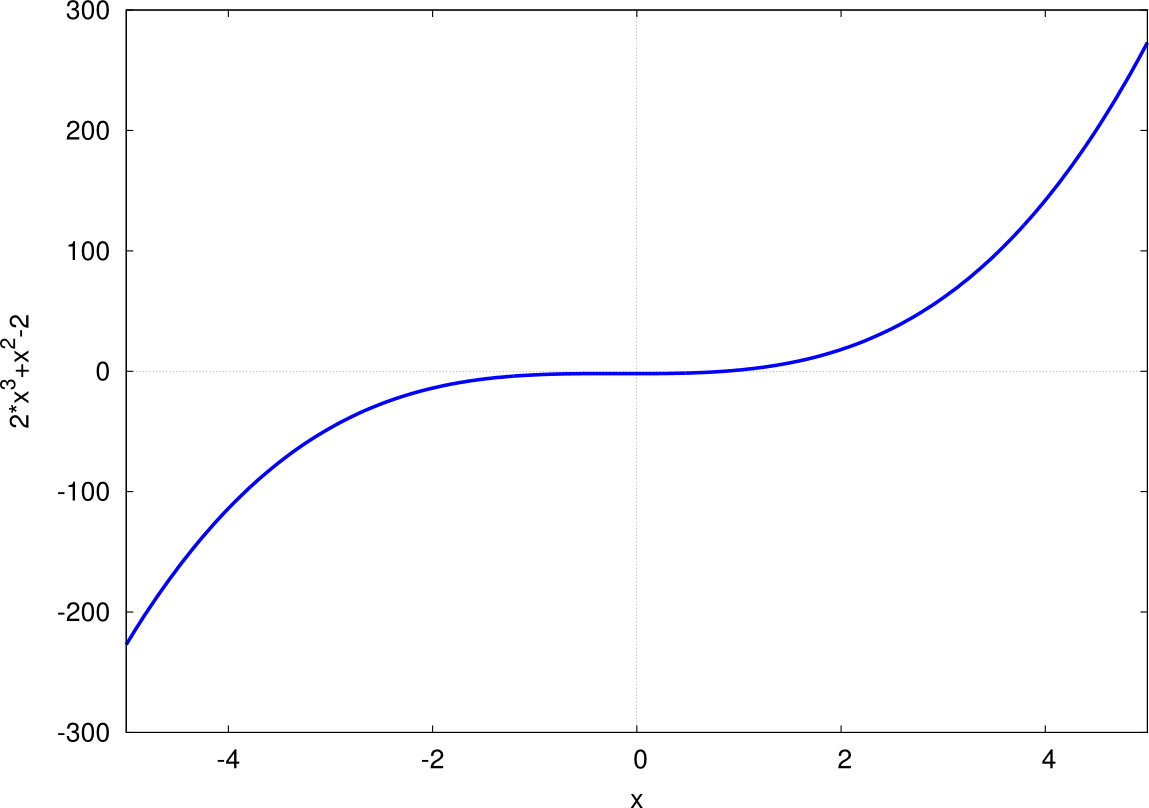
\includegraphics[scale = 0.5]{plot.png}
 \caption{$f(x) = 2x^3 + x^2 -2$}
\end{figure}

\begin{figure}[H]\centering
 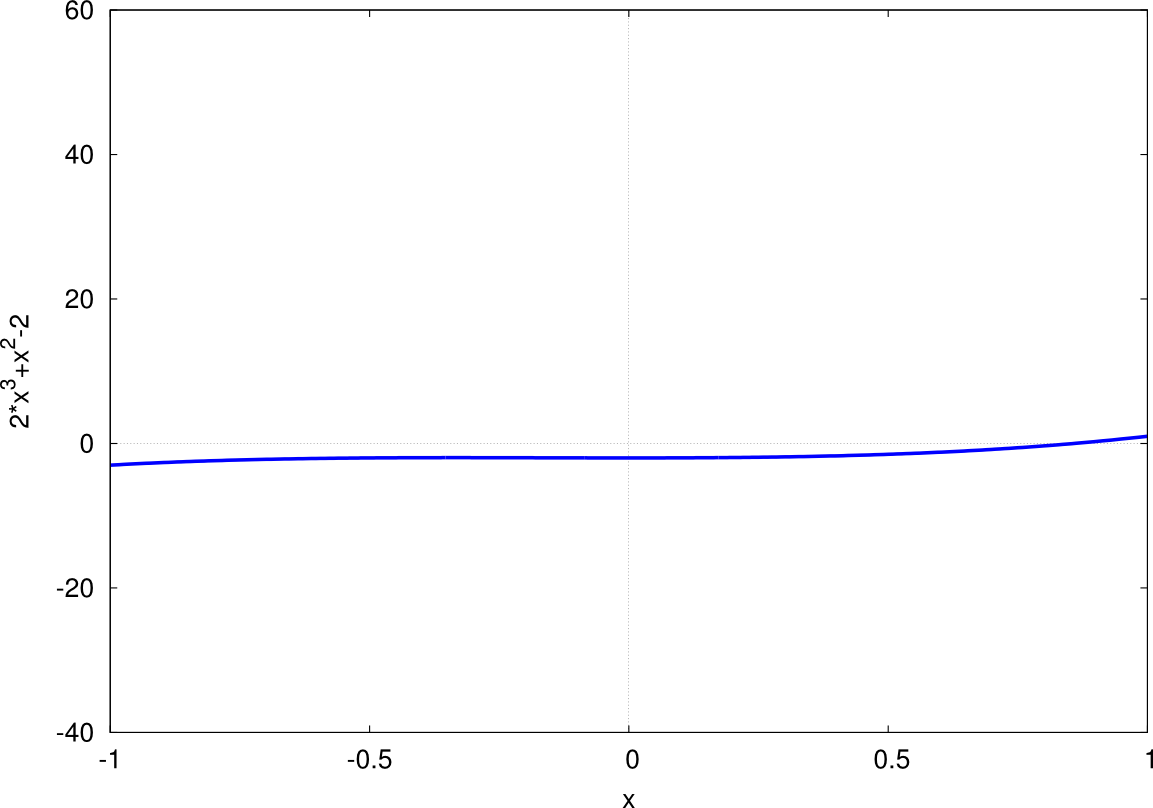
\includegraphics[scale = 0.5]{plot2.png}
 \caption{$f(x) = 2x^3 + x^2 -2$}
\end{figure}
Como podemos notar pelos gráficos expostos acima e pela Tabela~\ref{ex:convergencia}, que embora o método da secante tenha convergido para uma solução, o resultado retornando por este está incorreto. Isso ocorre, pois o Teorema~\ref{teo:convergencia_p0_newtonraphson} garante apenas que, sob as hipóteses aceitáveis, o método de Newton-Raphson (aqui, equivalentemente, estendido para o método da secante) convergirá se a aproximação inicial escolhida for suficientemente precisa.

Por outro lado, através ainda de uma análise da Tabela~\ref{ex:convergencia}, percebemos nitidamente que, de modo geral, o método de Newton-Raphson converge muito mais rápido do que os demais métodos apresentados. Isso deve-se ao fato de que o método de Newton-Raphson é, na maioria dos casos, \emph{quadraticamente convergente}, enquanto os outros não o são. Os conceitos de \emph{quadraticamente convergente} e
\emph{linearmente convergente} são definidos abaixo.

\begin{definition}
Seja $\{p_n\}^{\infty}_{n = 0}$ uma sequência que convirja para $p$, com $p_n \neq p$ para todo $n$. Se existem cosntantes positivas $\lambda$ e $\alpha$ com \[\limit{n}{\infty}{\frac{|p_{n+1} - p|}{|p_n - p|^{\alpha}}} = \lambda\text{,}\]
então $\{p_n\}^{\infty}_{n = 0}$ \emph{converge para $p$ com ordem $\alpha$.}
 \end{definition}

\begin{definition}
Uma técnica iterativa da forma $p_n = g(p_{n-1})$ é dita da \emph{ordem $\alpha$} se a sequência $\{p_n\}^{\infty}_{n = 0}$ convergir para a solução $p = g(p)$ com ordem $\alpha$.
 \end{definition}

De modo geral, uma sequência com alta ordem de convergência converge mais rápido do que uma com menor ordem de convergência (ou seja, se $\alpha_1 > \alpha_2$, onde $\alpha_1$ é a ordem de convergência uma determinada sequência $\{p_n\}^{\infty}_{n = 0}$ e $\alpha_2$ é a odem de convergência de uma outra sequência $\{q_n\}^{\infty}_{n = 0}$, então espera-se que $\{p_n\}^{\infty}_{n = 0}$ convirja mais rapidamente do que $\{q_n\}^{\infty}_{n = 0}$). Temos dois casos especiais de ordem de convergência, os quais são expostos abaixo:

\begin{itemize}
\item Se $\alpha = 1$, dizemos que a sequência é \emph{linearmente convergente}.
\item Se $\alpha = 2$, dizemos que a sequência é \emph{quadráticamente convergente}.
\end{itemize}

Já o método da secante possui \emph{convergência supralinear}, isto é, \[1 < \alpha < 2\text{.}\] Mais precisamente, neste caso, \[\alpha = \frac{1}{2}\sqrt{1 + \sqrt{5}} \approx 1.6818\text{.}\]

\section{Implementações}

Por fim, apresentaremos nesta seção uma implementação dos algoritmos expostos acima. Optamos utilizar a \emph{linguagem C} para este feito, devido a mesma ser uma linguagem de mais baixo nível (se comparado com as demais linguagens usuais como \emph{Java}, \emph{Python}, etc.), o que interfere diretamente, de forma positiva, no desempenho da execução do programa. 

Tais implementações foram feitas seguindo a risca (com pequenas \textquotedblleft modificações\textquotedblright apenas por conta da linguagem utilizada e da apresentação gŕafica dos resultados) os algoritmos expostos ao longo deste trabalho. Cada implementação possui os respectivos métodos para determinar $f(x) = 0$, dada a função $f(x)$. Além desta determinação, a cada passo da execução dos métodos é gerado um gráfico da função $f(x)$ e o respectivo ponto $(x, f(x))$ para o qual $f(x) = 0$ (caso este seja determinado pelo método executado). 

Ademais, para cada método foram feitas duas implementações, uma para quaisquer $f(x)$ que são funções polinomiais, onde o usuário entra via teclado com o valor de $f(x)$ e outra implementação para quaisquer funções $f(x)$ aceita pela biblioteca do C \emph{math.h}. No entanto, se nesta última implementação $f(x)$ for alterado, então esta implementação deve ser sempre recompilada com a nova função $f(x)$ e, no caso do Newton-Raphson, também com a função $f'(x)$ correspondente. Segue abaixo cada uma dessas implementações.
   
  \codC\lstinputlisting[caption = {newtonRaphson.c}]{../newtonRaphson.c}
  
  \codC\lstinputlisting[caption = {WithDefines/newtonRaphson.c}]{../WithDefines/newtonRaphson.c}
  
  \codC\lstinputlisting[caption = {bissecao.c}]{../bissecao.c}

  \codC\lstinputlisting[caption = {WithDefines/bissecao.c}]{../WithDefines/bissecao.c}
  
  \codC\lstinputlisting[caption = {falsaPosicao.c}]{../falsaPosicao.c}

  \codC\lstinputlisting[caption = {WithDefines/falsaPosicao.c}]{../WithDefines/falsaPosicao.c}
  
  \codC\lstinputlisting[caption = {secante.c}]{../secante.c}

  \codC\lstinputlisting[caption = {WithDefines/secante.c}]{../WithDefines/secante.c}

%==============================================================================================================

%Bibliografia=================================================================================================
 \renewcommand{\refname}{Referências Bibliográficas} 
 
 %\clearpage\thispagestyle{empty}\cleardoublepage
 \nocite{*}
 \bibliographystyle{plain}
 \addcontentsline{toc}{section}{Referências Bibliográficas}
 \bibliography{bibliografia_}
%==============================================================================================================

\end{document}
